\documentclass[12pt]{article}
\usepackage[margin=2.5cm]{geometry}
\usepackage{enumerate}
\usepackage{amsfonts}
\usepackage{amsmath}
\usepackage{fancyhdr}
\usepackage{amsmath}
\usepackage{amssymb}
\usepackage{amsthm}
\usepackage{mdframed}
\usepackage{graphicx}
\usepackage{subcaption}
\usepackage{adjustbox}
\usepackage{listings}
\usepackage{xcolor}
\usepackage{courier}
\usepackage[utf]{kotex}
\usepackage{hyperref}
\usepackage{soul}
\usepackage{cancel}


\definecolor{codegreen}{rgb}{0,0.6,0}
\definecolor{codegray}{rgb}{0.5,0.5,0.5}
\definecolor{codepurple}{rgb}{0.58,0,0.82}
\definecolor{backcolour}{rgb}{0.95,0.95,0.92}

\lstdefinestyle{mystyle}{
    backgroundcolor=\color{backcolour},
    commentstyle=\color{codegreen},
    keywordstyle=\color{magenta},
    numberstyle=\tiny\color{codegray},
    stringstyle=\color{codepurple},
    basicstyle=\ttfamily\footnotesize,
    breakatwhitespace=false,
    breaklines=true,
    captionpos=b,
    keepspaces=true,
    numbers=left,
    numbersep=5pt,
    showspaces=false,
    showstringspaces=false,
    showtabs=false,
    tabsize=1
}

\lstset{style=mystyle}

\pagestyle{fancy}
\renewcommand{\headrulewidth}{0.4pt}
\lhead{CSC 369}
\rhead{Reading Notes}

\begin{document}
\title{CSC 369 Reading Notes}

\section{Process}

\begin{mdframed}
\underline{\textbf{Vocabularies}}

\bigskip

\begin{enumerate}[1.]
    \item \textbf{Process}
    \begin{itemize}
        \item Is a program in execution
    \end{itemize}
    \item \textbf{Running Program}
    \begin{itemize}
        \item Is a collection of coded software instructions that can be executed
        by a computer to perform a specific task
    \end{itemize}
    \item \textbf{Time Sharing}
    \begin{itemize}
        \item Is a basic technique used by an OS to share a resource
        \item Allows an entity to use the resource for a little while, and then
        a little while by another, and so forth

        \bigskip

        \underline{\textbf{Example}}

        \bigskip

        CPU

    \end{itemize}
    \item \textbf{Space Sharing}
    \begin{itemize}
        \item Is where a resource (space) is divided among those who wishes to use it

        \bigskip

        \underline{\textbf{Example}}

        \bigskip

        Disk, and Memory
    \end{itemize}
    \item \textbf{Mechanism}
    \begin{itemize}
        \item Is a low-level method or protocol that implement a needed piece of
        functionality.

        \bigskip

        \underline{\textbf{Example}}

        \bigskip

        Context Switching
    \end{itemize}
    \item \textbf{Policy}

    \begin{itemize}
        \item Is an algorithm for making some kinds of decision within the OS

        \bigskip

        \underline{\textbf{Example}}

        \bigskip

        Scheduling Policy. That is, what kind of program should the OS run?
    \end{itemize}
    \item \textbf{Address Space}
    \begin{itemize}
        \item Is a range of discrete addresses where each corresponds to a memory cell

        \bigskip

        \begin{center}
        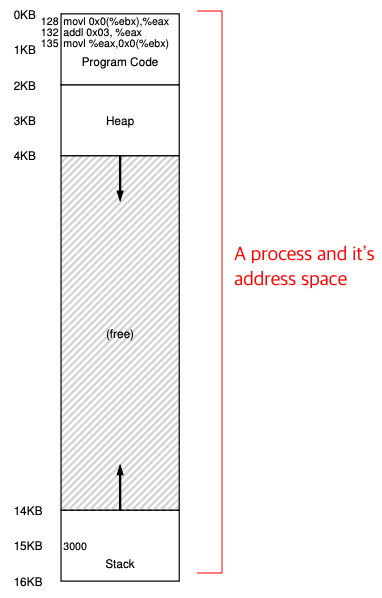
\includegraphics[width=0.5\linewidth]{images/notes_4_1.png}
        \end{center}

    \end{itemize}
    \item \textbf{Program Counter}
    \begin{itemize}
        \item Is also called \textbf{Instruction Pointer}
        \item Is a process register that tells which instruction of the program
        is currently being executed
    \end{itemize}
    \item \textbf{Stack Pointer}
    \begin{itemize}
        \item Is a resgister that points to the location of last item placed in memory block

        \begin{center}
        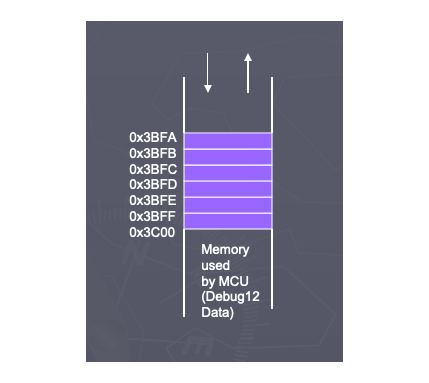
\includegraphics[width=0.5\linewidth]{images/notes_4_2.png}
        \end{center}
    \end{itemize}
    \item \textbf{Frame Pointer}
    \begin{itemize}
        \item Is a reference pointer allowing a debugger to know where local
        variable or an argument is at with a single constant offset

        \begin{center}
        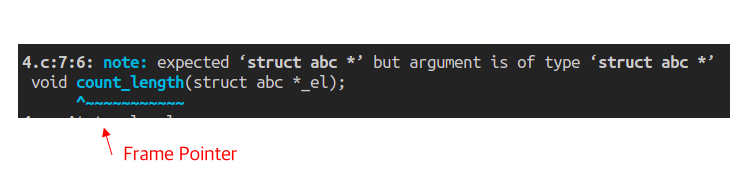
\includegraphics[width=0.8\linewidth]{images/notes_4_3.png}
        \end{center}
    \end{itemize}
    \item \textbf{Eager Loading Process}
    \begin{itemize}
        \item Is the process that loads all code and data before running the program
    \end{itemize}
    \item \textbf{Lazy Loading Process}
    \begin{itemize}
        \item Is the process that loads piece of code or data only as they are needed during
        program execution
    \end{itemize}
    \item \textbf{Stack}
    \begin{itemize}
        \item Is also called \textbf{runtime stack}, \textbf{automatic memory}
        \item Is a special region in computer's memory that temporarily stores local variables,
        function parameters, and return addresses
        \item Is managed by compiler
    \end{itemize}
    \item \textbf{Heap}
    \begin{itemize}
        \item Is a user-managed region in computer memory
        \item Is used for dynamically-allocated data structures such as linked list, hash-tables, and trees
        \item Is allocated using \texttt{malloc}, \texttt{calloc}, and \texttt{realloc}
    \end{itemize}
    \item \textbf{File Descriptors}
    \begin{itemize}
        \item Is a number that uniquely identifies an open file in a computer's operating system

        \begin{center}
        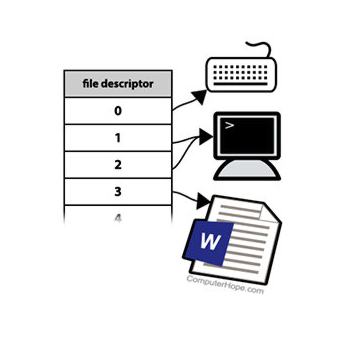
\includegraphics[width=0.5\linewidth]{images/notes_4_4.png}
        \end{center}
    \end{itemize}
    \item \textbf{Process States}
    \begin{itemize}
        \item Is also called \textbf{kernel state}
        \item Is the state field in a \textbf{process control block}.

        \bigskip

        \underline{\textbf{Example}}

        \bigskip

        \texttt{Ready, Running, Blocked}
    \end{itemize}
    \item \textbf{Process List}
    \begin{itemize}
        \item Is also called \textbf{task list}
        \item Contains information about all the processes running in the system
        \item Contains \textbf{process control block} in each entry
    \end{itemize}
    \item \textbf{Context Switch}
    \begin{itemize}
        \item is the process of storing the state of a process or thread, so
        that it can be restored and resume execution at a later point
    \end{itemize}
    \item \textbf{Register Context}
    \begin{itemize}
        \item Is the data structure where contents of registers are saved before
        a process switches into blocked state

        \bigskip

        \begin{center}
        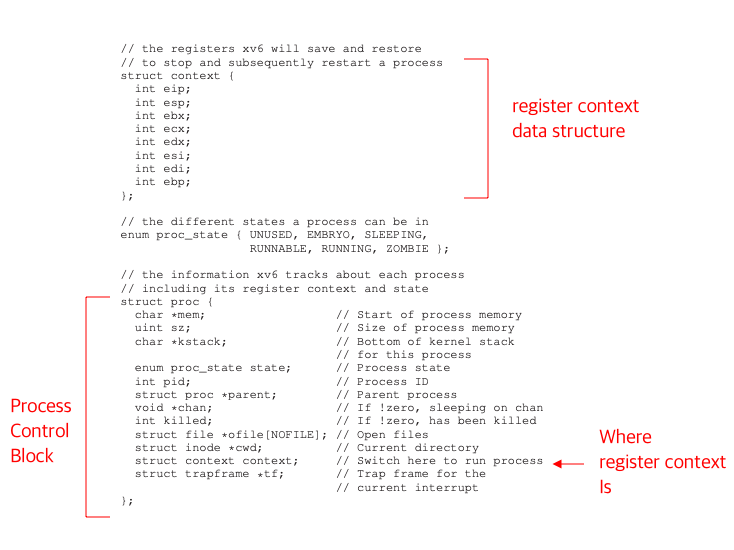
\includegraphics[width=0.8\linewidth]{images/notes_4_5.png}
        \end{center}

    \end{itemize}
    \item \textbf{Process Control Block}
    \begin{itemize}
        \item Is also called \textbf{process descriptor}
        \item Is a data structure used by computer operating systems to store all the information about a process
    \end{itemize}
    \item \textbf{Zombie State}
    \begin{itemize}
        \item Is a process that has completed execution but still has an entry in the process table
    \end{itemize}
\end{enumerate}

\end{mdframed}

\bigskip

\subsection{Process}
\begin{itemize}
    \item Is named by process ID or PID
    \item Is comprised of
    \begin{itemize}
        \item \textbf{Address Space}
        \item \textbf{CPU Registers}
        \item \textbf{Program Counter}
        \item \textbf{Stack Pointer}
        \item \textbf{Frame Pointer}
        \item \textbf{I/O Information}
    \end{itemize}
\end{itemize}

\subsection{Process API}
\begin{itemize}
    \item has the following methods in any operating systems
    \begin{itemize}
        \item \textbf{Create}
        \begin{itemize}
            \item Is a method for creating a new process
            \item Invoked to OS when
            \begin{itemize}
                \item A command is typed into shell
                \item An application icon is double-clicked
            \end{itemize}
        \end{itemize}
        \item \textbf{Destroy}
        \begin{itemize}
            \item Is a method for forcefully destroying a process

            \bigskip

            \underline{\textbf{Example}}

            \bigskip

            \texttt{kill}
        \end{itemize}
        \item \textbf{Wait}
        \begin{itemize}
            \item Is a method that causes a process stop running until a
            signal is given
        \end{itemize}
        \item \textbf{Miscellaneous Control}
        \item \textbf{Status}
        \begin{itemize}
            \item Is a method for getting information about a process

            \bigskip

            \underline{\textbf{Example}}

            \bigskip

            How long it has run for, what state it is in
        \end{itemize}
    \end{itemize}
\end{itemize}
\subsection{Process Creation: A little more detail}


\begin{itemize}
    \item Steps
    \begin{enumerate}[1.]
        \item Type a command into commandline / Double click an application
        \item Load program code and static data (e.g. initialized variables) into
        memory, into the address space of the process
        \item Allocate stack memory
        \item Allocate heap memory (if applicable)
        \item Setup I/O
        \begin{itemize}
            \item Each process has 3 open \textbf{file descriptors} by default:
            input, output and error
            \item Allows easy reading of input from the terminal and output to screen
        \end{itemize}
    \end{enumerate}

    \begin{center}
    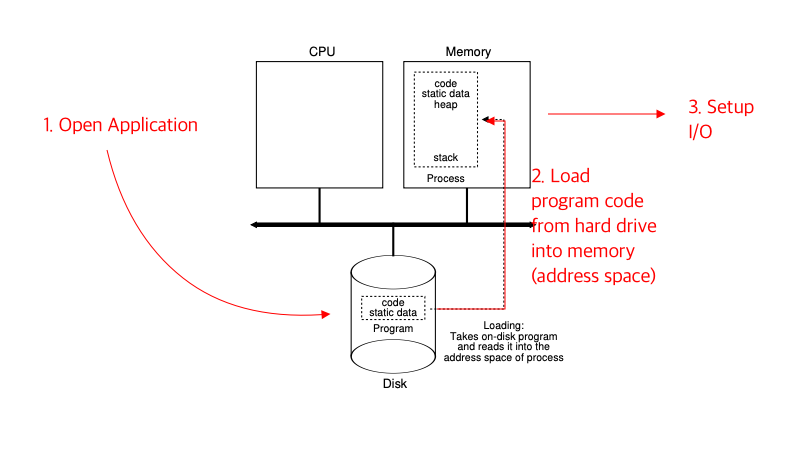
\includegraphics[width=0.4\linewidth]{images/notes_4_6.png}
    \end{center}

    \item \textbf{Eagerly loading process} in early days
    \item \textbf{Lazy loading process} today
\end{itemize}
\subsection{Process States}

\begin{itemize}
    \item A \textbf{process} is in one of three states
    \begin{itemize}
        \item \textbf{Running}
        \begin{itemize}
            \item Means a process is running on a processor. That is, coded instruction
            is being executed.
        \end{itemize}
        \item \textbf{Ready}
        \begin{itemize}
            \item
        \end{itemize}
        \item \textbf{Blocked}
    \end{itemize}
\end{itemize}

\subsection{Data Structures}

\end{document}
